\documentclass[11pt]{article}

\usepackage{graphicx}

\begin{document}
\title{CS344 Final: POSIX APIs and their Windows counterparts}
\author{Elliott Capek}
\maketitle

POSIX is a body of rules which specify an interface an operating system can provide to allow programmers to write portable programs. The actual implementation of the interface differs from OS to OS, but any POSIX-adopting OS's interface must have the same behavior. POSIX describes how programs interact with the file system and devices, how processes can access memory, OS information and communicate with each other, how processes can create new processes or threads, and many other things. \\ \\
This document will summarize the following POSIX APIs: memory mapping with \textbf{mmap}, thread creation with \textbf{pthreads}, interprocess communication with \textbf{sockets} and process creating with \textbf{fork}. It will also explain analogous Windows versions of these APIs and how they are different.\\

\section{Sockets}
Sockets are a tool in POSIX that can be used to communicate between processes. A socket is similar to a pipe in that, once two processes have succesfully opened their respective sockets and connected them, reads and writes can be done to the socket and the communication ``just works''. However, this is just one type of socket, known as a Stream Socket. The other major type is called a Datagram Socket, which is different in that individual buffered messages are packaged and sent, and the socket behaves less like a file. A more important difference between sockets and pipes is that sockets are not bound to the same operating system. When a socket is created it is given a protocol to use. The two major ones are the Unix domain and the Inet/Inet6 domain. The former is for communication within the same file system, while the latter is used for communication between networked machines over the internet. Sockets are the major way traffic is sent over the internet. HTTP, SSH, and other important programs/tools use sockets to achieve their inter-machine communication.

\subsection{Sockets in POSIX}
POSIX sockets all have a file descriptor they correspond to. In order to create a new socket for communication, the \textbf{socket(domain, type, protocol} system call must be used.\\ \\
\textbf{domain} refers to the protocol to be used (local or internet communication).\\ \\
\textbf{type} refers to the type of socket to be used: stream or datagram. Stream sockets are byte-streams. This means that read() and write() calls are used to send messages. Write() blocks until there is enough room in the socket buffer to hold the message. Read blocks until data has been written by the other socket holder. Closing the socket sends an EOF. Reading an EOF also closes the socket. Byte-streams are not conventional files. The lseek() command cannot be used on them, since data is destroyed once it is read. In a byte-stream, there is no concept of ``messages'' - data is written serially. This contrasts with the datagram socket, where messages are passed individually via send and receive calls. Datagram sockets do not guarantee messages are actually sent, or arrive in order. \textbf{protocol} is for future use, and currently has no influence on behavior. It should be 0.\\ \\

\begin{figure}[h!]
\centering
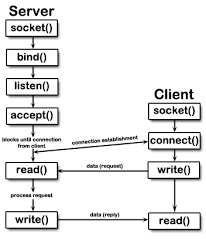
\includegraphics[width=0.5\textwidth]{socket-chronology.png}
\caption{Diagram of chronology of a typical streaming socket connection between a client and server. Image courtesy http://www.cs.uregina.ca/Links/class-info/330/Sockets/sockets.html and ``Unix Network Programming'' by W. Richard Stevens.}
\label{fig:socket-chronology}
\end{figure}

Once a socket has been created, there is a default timeline of events for communication. Typically one process acts as the server, which opens a named socket and waits for a client process to connect. This chronology is shown in Figure (\ref{fig:socket-chronology}). First, \textbf{bind()} is used to give the socket a name. In local communication, this is typically a filename. For internet communication, this is a port. Other processes use this port, along with your computer's host name, to connect. Once the socket is bound, \textbf{listen()} is called to tell the kernel this socket is ready for a connection. After this, two things must happen, and they can happen in any order. The server must \textbf{accept()} a connection request, and a client must initiate a \textbf{connect()} request. The first call blocks until the second call occurs (sort of like a telephone call: one caller blocks until the other answers, or a timeout occurs). The \textbf{accept()} call returns the file descriptor of a new socket which is connected to the client application. Reading and writing (or sending and receiving) can now occur on the two sockets.\\ \\
An interesting thing to note is that in POSIX, a socket is actually two different byte streams: one for reading and one for writing, just like a bidirectional pipe. One process implicitly writes to its write fd and reads from its read fd, even though only one socket file descriptor is used. This behavior is handled by the kernel. \\

\subsection{Sockets in Windows: WinSock}
WinSock, the Windows implementation of sockets, is very similar to the POSIX implementation. There are \textbf{socket()}, \textbf{bind()}, \textbf{listen()}, \textbf{accept()}, \textbf{connect()}, \textbf{recv()} and \textbf{send()} calls which work in a very similar way to the POSIX calls. There are some calls with different names, such as \textbf{closesocket()}. The fact that the \textbf{close()} system call cannot be used on WinSock sockets is a result of WinSock sockets not actually being files, but different sorts of data structures. Windows does not have the ``everything is a file'' paradigm that Unix adopts. This is an advantage in that it puts sockets in a totally different namespace than files, so collisions are less likely. However, it limits users to only using the WinSock API to use sockets, instead of using other APIs to interact with the actual file, like in POSIX. Using non-socket APIs to interact with sockets probably is not very useful, but there may be some cases when it is nice. Another necessary function when using sockets in Windows is the \textbf{WSAStartup()} call, which must be used before any other socket calls are run. This function loads the Windows Sockets DLL (shared library). This is very different than the way POSIX does things, where shared libraries are automatically loaded. This gives more power to the programmer, since it allows them to specify versions and things explicitly. However, it also may cause a performance drop, since DLLs probably take time to load. As expected, the \textbf{WSACleanup()} function must be called after sockets are done being used to unload the DLL.\\

\subsection{POSIX vs Windows}
As described above, there are many shared system calls between POSIX and Windows. One of the most notable differences is that, because Windows sockets are not files, \textbf{write()} and \textbf{read()} do not work on Windows sockets. Everything is done through calls to \textbf{recv()} and \textbf{send()}. This allows for less versatility (treating sockets like files makes many things easy in POSIX, like piping a command to a socket) but potentially more confusion, since many of the read() and write() flags used on files do not work on sockets. One thing that is immediately obvious when looking at the MSDS documentation for Windows Sockets is that Windows provides a huge number of socket-specific functions: functions to resolve host names via DNS, simultaneously open and read socket connections, send files over sockets, etc. These are some very powerful API calls that make programming in Windows nice.\\

\section{Memory Mapping}
Memory mapping is the act of creating linkages between regions in a program's memory and external data structures, either files or anonymous spaces in memory. This is incredibly convenient, since it allows programs to write to files as if they were memory (random access via pointers, memset, etc..). It also allows two processes to conveniently share large portions of data, since multiple processes can map their private memory to shared files or anonymous structures. There are two types of mappings: private and shared. The difference is intuitive: only one process can access a private mapping, whereas many processes can access a shared mapping. A private file mapping is a single process taking ownership of a file and using it. If another process maps this file, the kernel assures that changes made by other processes are invisible to to each process. This is used to initialize memory from a file. Private anonymous mappings allocate memory that only the calling process can use. Private anonymous mappings are very similar to malloc() calls. Shared file mappings allow multiple processes to easily and quickly use and modify the same set of data. Shared anonymous mappings use memory that is within the parent process's memory space, and so only children can access it, not other processes.\\

\subsection{POSIX Memory Mapping}









\end{document}



References:
http://johnnie.jerrata.com/winsocktutorial/
https://msdn.microsoft.com/en-us/library/windows/desktop/ms740632(v=vs.85).aspx
